\documentclass[]{politex}

% ========== Packages ==========
\usepackage[utf8]{inputenc}
\usepackage{amsmath,amsthm,amsfonts,amssymb}
\usepackage{graphicx,cite,enumerate}
\graphicspath{ {./images/} }
\usepackage{tabularx}

% ========== Language options ==========
\usepackage[brazil]{babel}
%\usepackage[english]{babel}


% ========== ABNT (requer ABNTeX 2) ==========
%	http://www.ctan.org/tex-archive/macros/latex/contrib/abntex2
\usepackage[num]{abntex2cite}

% Forçar o abntex2 a usar [ ] nas referências ao invés de ( )
\citebrackets{[}{]}


% ========== Lorem ipsum ==========
\usepackage{blindtext}

% ========== Opções do documento ==========
% Título
\titulo{Rede de Dipositivos para Monitoramento de qualidade e conforto em escritórios}

% Autor
\autor{Isabella Bologna Salomão\\%
		Renato de Oliveira Freitas}


% Orientador / Coorientador
\orientador{Prof. Dr. Gustavo P. Rehder\\%
			Prof.ª Dra. Cíntia Borges Margi}
\coorientador{PullUp \\%
            Eng. Conrado Leite de Vitor }

% Tipo de documento
%\tcc{Eletricista com ênfase em Eletrônica e Sistemas}
\tccp
%\dissertacao{Engenharia Elétrica}
%\teseDOC{Engenharia Elétrica}
%\teseLD
%\memorialLD

% Departamento e área de concentração
\departamento{PCS - Computação e Sistemas Digitais}
%\areaConcentracao{Área de concentração}

% Local
\local{São Paulo}

% Ano
\data{2020}


\begin{document}
% ========== Capa e folhas de rosto ==========
\capa
\folhaderosto


% ========== Resumo ==========
\begin{resumo}
Soluções para o monitoramento de parâmetros que remetem à qualidade e conforto de ambientes internos vêm se tornando interessantes, dado o aumento no tempo que pessoas passam nesse tipo de ambiente, como escritórios. A partir da coleta desses dados, é possível adotar medidas para tornar o local estudado mais saudável e confortável para as pessoas ali presentes. O objetivo desse trabalho é desenvolver uma rede de dispositivos eletrônicos \textit{Open Source} capaz de monitorar escritórios fechados, realizando a medição através de sensores de dados referentes à qualidade do ar, temperatura, luminosidade e ruído, e coletando a opinião das pessoas sobre sua sensação de conforto no ambiente, para apresentar relatórios sobre o local em uma plataforma a fim de tomar ações para garantir o conforto de seus ocupantes. 
%
\\[3\baselineskip]
%
\textbf{Palavras-Chave} -- Internet of Things, Conforto Térmico, Conforto Acústico, Conforto Luminoso, Qualidade do Ar, Wireless Sensor Network, Green Buildings, Smart Office.
\end{resumo}


% ========== Sumário ==========
\sumario

% ========== Elementos textuais ==========

\chapter{Introdução}

\section{Declaração da Necessidade}
% Contexto, PCC

Com o aumento do tempo que as pessoas passam em ambientes fechados, como escritórios, há também, nos últimos anos, um crescente interesse em monitorar e controlar tais ambientes, visando uma melhora na saúde e conforto das pessoas, e também um aumento na sua produtividade. Espaços que implementam essas soluções são comumente chamados de prédios inteligentes (\textit{smart buildings}, do inglês). É possível até mesmo que esse controle seja utilizado para uma atuação de maneira energeticamente sustentável e, dentro desse conntexto, surgem os \textit{green buildings} (em português, construções sustentáveis) \cite{GreenBuildings} \cite{EnergyBuildings}.

No desenvolvimento de construções civis sustentáveis, torna-se necessário que seja pensada a implementação automatizada deste monitoramento dos ambientes desde o projeto da edificação e sua concepção, ocorrendo de forma integrada à construção. Uma pesquisa mais aprofundada sobre o conforto dos ambientes pode interferir no projeto, de modo que sejam repensados materiais utilizados e sistemas de aquecimento, ventilação, iluminação, dentre outros. Assim como a sua implementação, pesquisas na área de conforto têm ser tornado cada vez mais importantes. 

Foi com essa necessidade e a proposta de desenvolver um dispositivo eletrônico que o professor Vanderley M. John, do departamento de Construção Civil da Poli (PCC) e coordenador do CICS (Centro de Inovação em Construção Sustentável da USP)\cite{CICS}, entrou em contato. A ideia é que seja desenvolvido um dispositivo capaz de fazer medições de parâmetros relacionados ao conforto nos ambientes internos de uma construção, coletando também a opinião das pessoas ali presentes acerca de seu bem-estar, para assim saber o real impacto dos indicadores de conforto. Para analisar todo o ambiente, é importante que existam diversos dispositivos espalhados para maior cobertura. A fim de analisar ambos os dados (medições do ambiente e opiniões), é interessante que esses dispositivos estejam conectados e integrados a uma central. 

Assim, a construção de uma rede de dispositivos sensoreados tem, além de uma aplicação prática monitorando a qualidade para as pessoas, também grande utilidade em pesquisas de construção civil e arquitetura, com medições mais precisas e incluindo um elemento muitas vezes deixado de lado: o fator humano.

Em edifícios, escritórios são hoje os que ocupam a maior área física e tem o maior consumo de energia, sendo sistemas de iluminação, aquecimento e resfriamento (como ar condicionados) os principais causadores do alto consumo\cite{EnergyBuildings}. Por isso, escritórios são o nicho escolhido para a implementação dessa rede de dispositivos, podendo ser testada nas salas do departamento de Construção Civil ou do CICS. 


% Dificuldade em estudar elementos relacionados a conforto ?
% Falar do que já existe? 

\section{Descrição do Problema} % Requisitos

O conforto e a qualidade em ambientes internos são determinados através de quatro principais indicadores: \textbf{térmico, acústico, luminoso e olfativo/qualidade do ar}\cite{ComfortBox}. 

Para que seja possível monitorar esses indicadores, é necessário medirmos diversos dados a respeito do ambiente em questão: %%% ??  essa frase
\begin{itemize}
\item Térmico: temperatura ambiente e umidade relativa
\item Acústico: ruído ambiente
\item Luminoso: intensidade e temperatura da luz incidente
\item Qualidade do ar (e Olfativo): CO2 e VOC (\textit{volatile organic compounds})
\end{itemize}

Não apenas esses elementos são importantes, mas também a combinação deles afeta a percepção de conforto pelas pessoas \cite{ComfortOffice}. Assim, faz-se mais necessário que haja uma medição completa dos elementos presentes no ambiente a ser estudado. Além disso, é interessante que essas medições estejam atreladas a opinião das pessoas a respeito do ambiente, sabendo se estão confortáveis, sendo necessário um sistema que possa coletar um \textit{feedback} das pessoas no escritório. 

%Conectividade
Todos os dados coletados, tanto das variáveis do ambiente quanto a opinião das pessoas, precisam ser salvos e disponibilizados para análise. Assim, será necessária a existência de conectividade nos dispositivos, junto de uma plataforma em nuvem com um banco de dados e uma interface visual para que seja feita essa análise. 

\section{Árvore de Objetivos} 
% arvore de objetivos
A árvore de objetivos é uma representação gráfica dos meios necessários, chamados objetivos específicos, para alcançar o objetivo geral do projeto. Para atingir o objetivo geral do projeto, que é a realização de uma rede de dispositivos para monitorar ambientes, foram enunciados três objetivos específicos, mostrados na figura \ref{fig:objective-tree}, com a porcentagem de dedicação ao lado de cada um.

\begin{figure}[h!]
%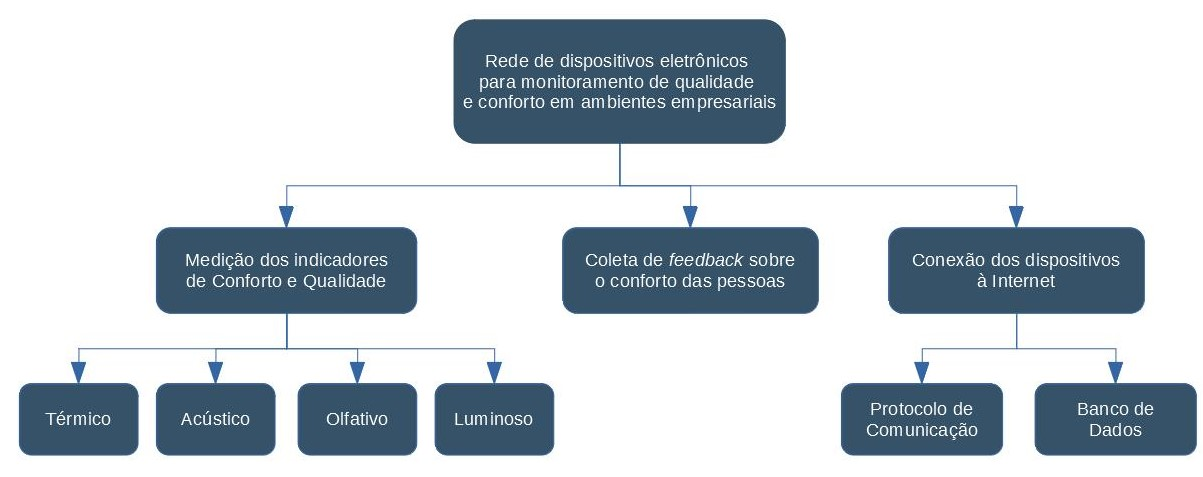
\includegraphics[scale=0.65]{objective_tree}
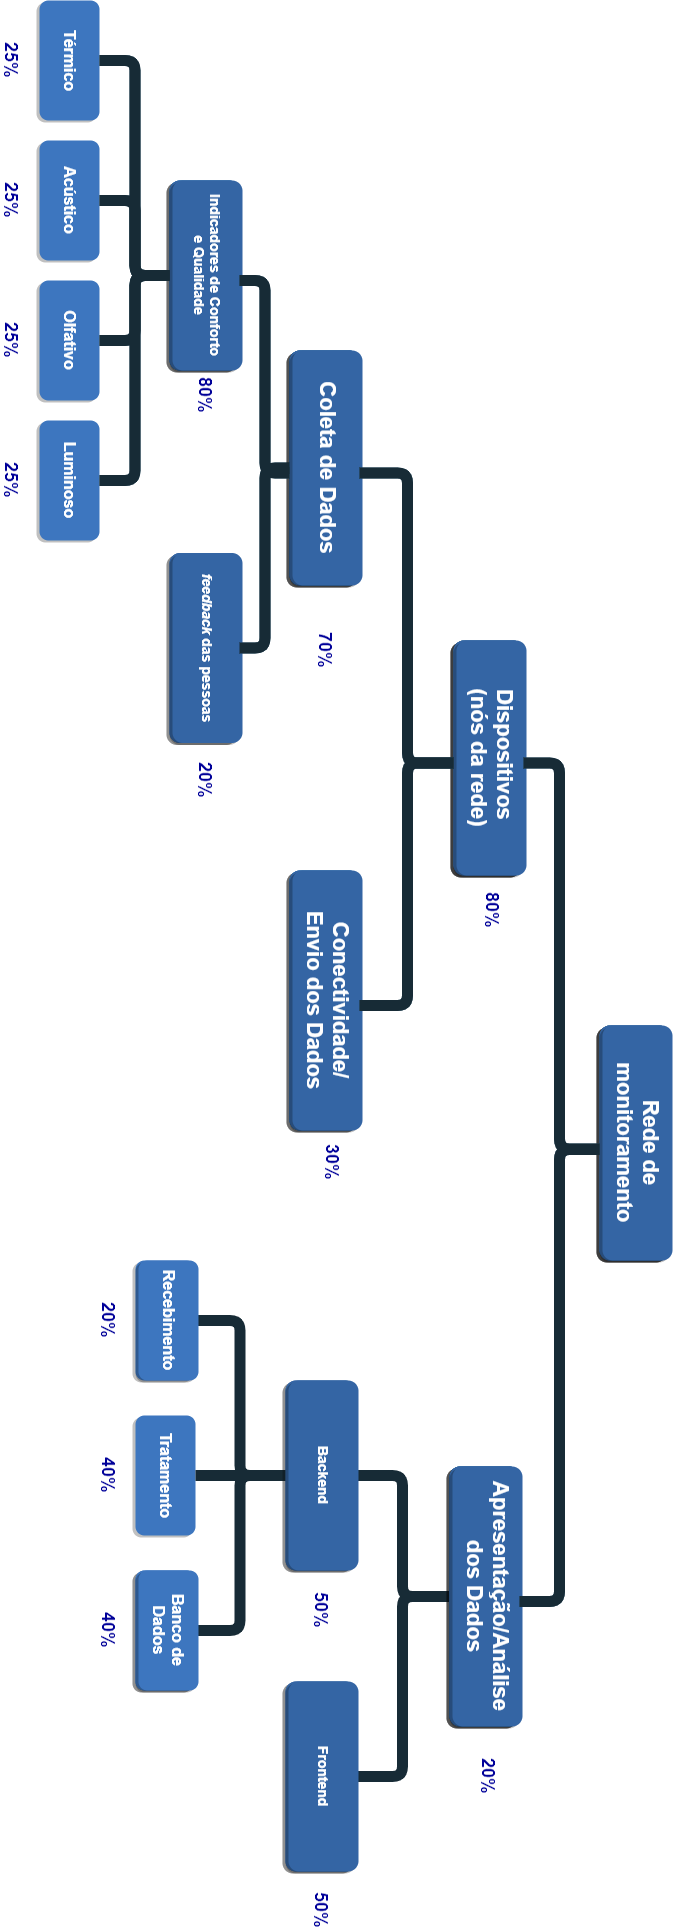
\includegraphics[width=\textwidth]{objective-tree-2}
\caption{Árvore de objetivos do projeto}
\label{fig:objective-tree}
\end{figure}

\chapter{Conforto em Ambientes Fechados} % Tema? ~Estado da Arte~

\section{Indicadores de Qualidade e Conforto} %?

% Separar qualidade e conforto

% Qualidade -> Limites pela legislação e pesquisas
Como qualidade e conforto são termos subjetivos, vamos tratar aqui como "qualidade do ambiente" as condições recomendadas por normas e pesquisas, para os quatro indicadores. Isto é, será considerado um ambiente de boa qualidade o que atender às faixas de operação pré-determinadas, funcionando como um aviso para o ocupante caso as medidas indiquem que os parâmetros do ambiente estão fora do recomendado. 

Já o conforto será atrelado à percepção do usuário quanto ao ambiente. Apesar de o ambiente ser considerado saudável ou de qualidade, existem muitos fatores que afetam a sensação das pessoas, de forma que apenas a definição de uma faixa de operação não implica em bem-estar. 
% citações ??

\subsection{Regulamentações e Normas} %check

A legislação brasileira determina os valores máximos e mínimos dos indicadores de conforto no ambiente para que haja boas condições de trabalho: 

\begin{citacaoLonga} %Normas ministerio
\textbf{NR17 do Ministério do Trabalho} \cite{NR17}

17.5. Condições ambientais de trabalho.

17.5.2. Nos locais de trabalho onde são executadas atividades que exijam solicitação intelectual e atenção constantes, tais como: salas de controle, laboratórios, escritórios, salas de desenvolvimento ou análise de projetos, dentre outros, são recomendadas as seguintes condições de conforto:

a) níveis de ruído de acordo com o estabelecido na NBR 10152, norma brasileira registrada no INMETRO;

b) índice de temperatura efetiva entre 20oC (vinte) e 23oC (vinte e três graus centígrados);

[...]

d) umidade relativa do ar não inferior a 40 (quarenta) por cento.

17.5.2.1. Para as atividades que possuam as características definidas no subitem 17.5.2, mas não apresentam equivalência ou correlação com aquelas relacionadas na NBR 10152, o nível de ruído aceitável para efeito de conforto será de até 65 dB (A)

[...]

17.5.3.3. Os níveis mínimos de iluminamento a serem observados nos locais de trabalho são os valores de iluminâncias estabelecidos na NBR 5413, norma brasileira registrada no INMETRO.
\end{citacaoLonga}

\begin{citacaoLonga} %Normas ABNT

\textbf{NBR 10152} \cite{NBR10152} para Escritórios

Salas de reunião: 30 - 40 dB(A)

Salas de gerência, Salas de projetos e de administração: 35 - 45 dB(A)

Salas de computadores: 45 - 65 dB(A)

Salas de mecanografia: 50 - 60 dB(A)

\textbf{NBR 5413} \cite{NBR5413}

Para escritórios: 500 - 750 - 1000 lux
\end{citacaoLonga}

\subsection{Conforto Visual} %check
Além da \textbf{intensidade da luz incidente}, cujos níveis são estabelecida na legislação, a \textbf{temperatura da cor} da luz incidente também tem grande relevância. A muitos anos sabe-se que a luz azul emitida, de maior temperatura, causa danos à retina \cite{BlueLight}. \par
Assim, temperatura é um parâmetro importante para a qualidade do ambiente, muitas vezes deixado de lado, e assim como na saúde, afeta diretamente o conforto e a atenção das pessoas, como visto em \cite{VisualComfort}: 
\begin{itemize}
\item Conforto, luz natural: 3000K - 6000K
\item Concentração: acima de 5300K 
\end{itemize}

\subsection{Qualidade do Ar} % Pesquisa CO2 e VOC

% Colocar o que é IAQ, falar sobre?
% Sindrome Predios doentes? -> Intro?
Não há, na legislação brasileira, informações sobre a qualidade do ar. Isto é, concentrações de CO2 e VOC. 

A norma a seguir fala a margem esperada, mas também sem recomendações de operação. 

\begin{citacaoLonga} % ISO IAQ
\textbf{ISO 16017-2:2003}

is applicable to the measurement of airborne vapours of VOCs in a concentration range of approximately 0,002 mg/m3 to 100 mg/m3 individual organic for an exposure time of 8 h
\end{citacaoLonga}

Por conta disso, vamos nos basear em estudos que tentam relacionar as concentrações de CO2 e de VOC com efeitos na saúde e produtividade das pessoas. 

\subsubsection{CO2}
Segundo \cite{AirQuality}, o CO2 apresenta concentrações mais altas em ambientes fechados, esperando-se entre 700 e 2000 ppm, em comparação a cerca de 400ppm em ambientes abertos em áreas urbanas\cite{co2Earth}. 

O CO2, além de ser um gás asfixiante e perigoso em altas concentrações (acima de 40000ppm), também pode afetar a saúde quando em níveis moderados (abaixo de 2000ppm). 
De acordo com o \textit{Winsconsin Department of Health Services}\cite{Winsconsin}, são os efeitos causados na saúde: 
\begin{itemize}
\item 250-400ppm: Normal, concentração ambientes abertos
\item 400-1,000ppm: concentração típica em lugares fechados com pessoas, com boa circulação de ar
\item 1,000-2,000ppm: pode causar cansaço e falta de ar
\item 2,000-5,000 ppm: dores de cabeça, sonolência, e falta de ar mais intensa. Baixa concentração, perda de atenção, aumento da frequência cardíaca, e náusea
\item 40,000 ppm: Pode causar séria insuficiência respiratória, danos permanentes ao cérebro, coma e até a morte
\end{itemize}

\subsubsection{VOC}
Compostos orgânicos voláteis, ou VOC (do inglês,\textit{Volatile organic compounds}, são partículas que ficam suspensas no ar, podendo vir de produtos (sintéticos ou naturais) utilizados no ambiente, como tintas, solventes, produtos de limpeza, perfumes que podem causar odor perceptível pelo ser humano\cite{AirQuality}.

A concentração esperada é entre 0.2 e 0.5 mg/m3, e mesmo que nem todos os compostos presentes no ar sejam nocivos à saúde, por precaução é recomendado que estes sigam: \cite{tecam}

\begin{tabular}{ |c|c| }
\hline
TVOC Level [mg/m3]	&   Level of Concern \\
\hline
Less than 0.3 mg/m3	 &  Low \\
0.3 to 0.5 mg/m3	&   Acceptable \\
0.5 to 1 mg/m3	 &  Marginal \\
1 to 3 mg/m3	 &  High \\
\hline
\end{tabular}

%A tabela feita por \cite{sensirion} mostra os níveis de TVOC aceitáveis (em ppb)
%\begin{tabular}{ |c|c| } 
%\hline
%TVOC [ppb] & Hygienic Rating\\ 
%\hline
%2200 to 5500 & Unhealty \\ 
%660 to 2200 & Poor \\ 
%200 to 660 & Moderate \\
%65 to 220 & Good \\
%0 to 65 & Excellent \\
%\hline
%\end{tabular}
%1 ppb = 1 mg/m3


\section{Soluções de Monitoramento} % ?? 
% Falar de ser Open Source

A tabela a seguir mostra algumas das principais soluções encontradas no mercado para monitoramento de ambientes fechados: 

\begin{center}
\begin{tabular}{ | m{2.5cm} | m{2.4cm}| m{2.2cm} |m{2cm} |m{2.1cm} |m{2.8cm} | } 
\hline
\textbf{Projeto} & \textbf{Térmico} & \textbf{Luminoso} & \textbf{Acústico} & \textbf{Ar} & \textbf{Conectividade} \\ 
\hline
Multi comfort \cite{multicomfort} & Sim* & Sim* & Sim* & Sim* & Sim* \\ \hline
MC350\cite{mc350} & Sim* & Sim* & Sim* & & Bluetooth, App \\
\hline
Metriful Sense\cite{metriful} & Temperatura, Umidade, Pressão & Intensidade & Volume, Frequência & VOC &  \\ \hline
CoMoS\cite{CoMoS} & Temperatura, Umidade, Veloc Ar & Intensidade & & & Wifi, SW Web \\ \hline
HC tech\cite{HCTech} & Temperatura, Umidade & Intensidade & & & Sigfox, SW Web \\ \hline
ECOMLITE \cite{ECOMLITE} & Temperatura, Umidade, Pressão & & Volume & CO2, VOC, CO, NO2 & Wi-fi, Zigbee, Ethernet, SW Web \\ \hline
Netatmo\cite{netatmo} & Temperatura, Umidade, & & Volume & CO2 & Wi-fi, App \\ \hline
Senlab O\cite{Senlab} & Temperatura, Umidade & Intensidade & & & LoRa \\ \hline
Comfort Click\cite{comfortclick} & Temperatura, Umidade & & Volume & & Wi-fi, App  \\ \hline
\end{tabular}
\end{center}

\begin{flushright}
(*) Solução não detalhada pela construtora
\end{flushright}


% Análise  - Finalizar
Ao observar as soluções existentes no mercado, é possível ver que a maioria atende a apenas alguns dos indicadores. 

Multi Comfort \cite{multicomfort}, a solução mais completa encontrada, trata-se de uma sistema desenvolvido pela construtora Saint-Gobain de forma integrada à construção do edifício. Como apresentado pelo prof. Vanderley (PCC), o monitoramento e automação na construção civil vem crescendo nos últimos anos, de forma que soluções desse tipo tendem a tornar-se mais comuns. 
Apesar de atender aos 4 indicadores de qualidade e conforto, essa solução não apresenta detalhes sobre as medições que são feitas, quais os elementos medidos ou a precisão dessas medições, assim como sobre a sua conectividade. Também apresenta grande dificuldade para integração em um ambiente já construído. Nesse contexto, é introduzido o equipamento MC350\cite{mc350} - da mesma empresa -, mas que não atende mais a todos os indicadores. 

Em seguida, temos o Metriful Sense \cite{metriful}, que também atende a todos os indicadores de conforto, que é um produto novo em \textit{crowdfunding}. Diferentemente das demais, esse não é um dispositivo completo, mas uma plataforma de sensores projetada para o monitoramento de ambientes, que necessita de uma interface com outro processador e possivelmente com um módulo \textit{wireless} para que haja conexão com uma plataforma de análise. 

Os demais produtos atendem em média apenas dois dos indicadores de conforto, sendo apenas o conforto térmico presente em todos. O conforto luminoso, quando presente, é atendido de forma superficial, sendo medida apenas a intensidade da luz e não a temperatura, que é um elemento importante na sensação de conforto \cite{VisualComfort}. Já no monitoramento da qualidade do ar, apenas uma das soluções \cite{ECOMLITE} (cuja especificação está disponível) mede ao menos os dois principais elementos indicadores \cite{AirQuality}. 

Vemos, assim, que nenhum dos produtos existentes no mercado atende a todos os requisitos levantados para a nossa aplicação. A proposta aqui é o desenvolvimento de um dispositivo que monitore a qualidade e o conforto do ambiente atendendo a todos os indicadores apresentados de forma completa, e com uma medição mais aprofundada em conforto luminoso e qualidade do ar que os projetos comparados. 

Além disso, nenhuma das soluções encontradas envolve diretamente a opinião das pessoas frequentando o ambiente na análise dos seus dados, apenas no controle do ambiente quando esse não atende os requisitos de qualidade ou de conforto. 

Vale destacar, por fim, que na maioria dos casos essas soluções são fechadas, com protocolos que dificultam a integração dos dispositivos com outros que possam complementá-los em seu funcionamento, ou de forma que seja possível uma centralização da análise dos dados coletados. Desenvolvendo um projeto \textit{open-source} e com protocolos padrão de comunicação sem fio, isso deixa de ser um problema. 


\chapter{Especificação Técnica}

\section{Arquitetura do Dispositivo} % Como atingir os objetivos (requisitos) e apronfunda specs da descrição do problema (especificação inicial)

\begin{figure}[h!]
    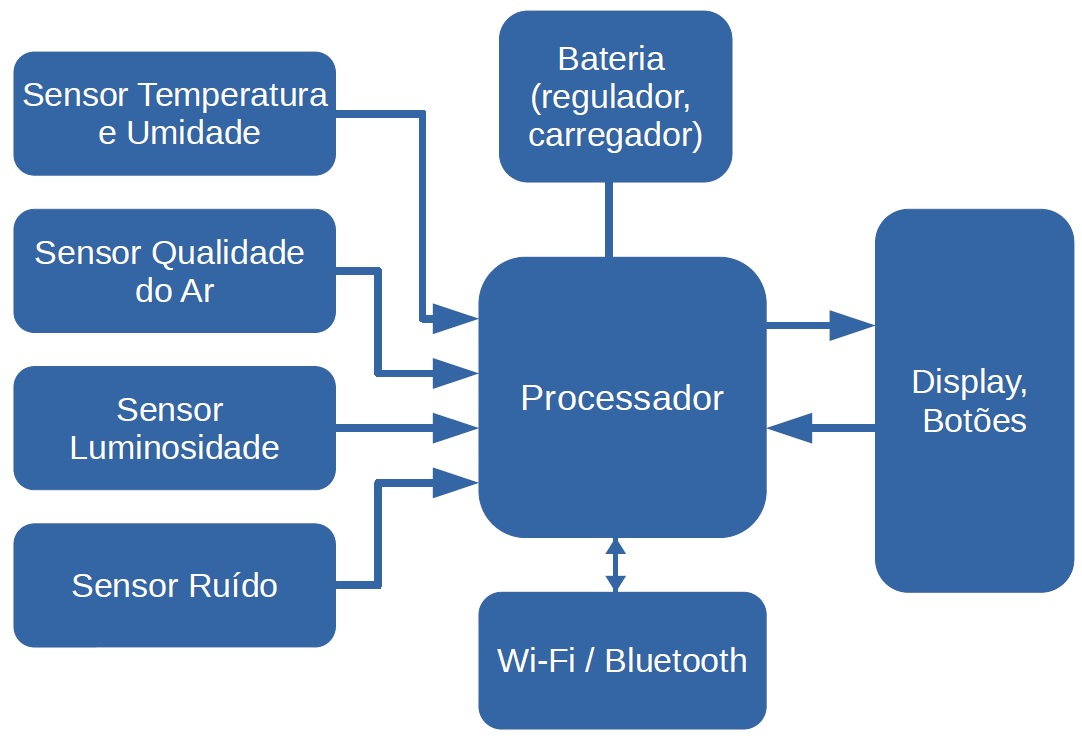
\includegraphics[width=\textwidth]{block_diagram}
    \caption{Diagrama de Blocos do Hardware do Dispositivo}
    \label{fig:Diagrama de Blocos}
\end{figure}

\subsection{\textit{System-on-a-Chip}}

\textit{System-on-a-Chip}, ou SoC, é o nome dado a um circuito integrado que engloba processador, periféricos, memória e outros módulos. Geralmente é desenvolvido em torno de um microcontrolador (ou um processador) integrando mais blocos, como de radiofrequência nesse caso, para comunicação sem fio.

Analisando as principais opções existentes no mercado de microcontroladores, para atuar como processador central do dispositivo, optamos por usar um ESP32. 

ESP32\cite{ESP32} é uma família de \textit{SoC}s da Espressif que possui um microcontrolador integrado às tecnologias Wi-Fi e Bluetooth. Por ter um bom suporte e ferramentas de desenvolvimento focadas em BLE e Wi-Fi, além de ter um dos menores preços, foi nossa escolha como melhor custo-benefício. 

 

\textbf{Especificações do ESP32:} \cite{ESP-datasheet}
\begin{itemize}
\item \textbf{Processador}: Xtensa 32-bits, dual core
\item \textbf{Wi-Fi}: 802.11 b/g/n
\item \textbf{Bluetooth}: v4.2 BR/EDR e BLE
\end{itemize}


\subsection{Sensores}
A fim de atender aos critérios apresentados para o monitoramento, foram escolhidos os seguintes sensores: 
\begin{itemize}
\item \textbf{AS7262}, da AMS: 

Atende aos requisitos de medição de \textit{conforto luminoso}. 

\textbf{Medidas}: Intensidade e cor da luz incidente.

A cor da luz, nesse sensor, é medida através de 6 canais, correspondendo aos espectros de luz vermelha (650nm), laranja (600nm), amarela (570nm), verde (550nm), azul (500nm) e violeta (450nm), ao invés de simples RGB, com resolução de 16 bits.

\textbf{Comunicação}: I²C, SPI ou UART (configurável)

\item \textbf{BME680}, da Bosch: 

Atende tanto aos requisitos de \textit{conforto térmico} quanto de \textit{qualidade do ar}.

\textbf{Medidas}: Temperatura com precisão de ±1.0°C, umidade relativa com precisão de ±3\%, pressão, ±1 hPa, e VOC, através de um sensor MOX, que pode ser usado para estimar concentração de gases como Etanol, CO e Álcool. 

\textbf{Comunicação}: SPI ou I²C

\item \textbf{Microfone de Eletreto}:

Em conjunto com um circuito amplificador, atende aos requisitos de \textit{conforto acústico}. 

\textbf{Medida}: volume de ruído sonoro ambiente

\textbf{Comunicação}: Analógica, com precisão a depender do conversor analógico digital escolhido (CI externo)
\end{itemize}

\section{Arquitetura da Rede}

\subsection{Conexão de Dispositivos}
Como citado anteriormente, as medições realizadas pelos dispositivos precisam ser salvas e enviadas para algum local de armazenamento, para posterior análise, exigindo que seja estabelecido um protocolo de conexão. Com o crescimento do conceito de Internet das Coisas, novas tecnologias para conexão rápida, segura e fácil de dispositivos surgem.

Wi-Fi é uma família de tecnologias designadas para comunicação sem fio baseada no padrão IEEE 802.11, amplamente utilizada em redes de área local (em inglês \textit{local area network}, LAN) para prover acesso à internet. Essa tecnologia opera nas faixas de 2,4 e 5GHz, sendo que a primeira permite uma taxa de transmissão de até 600 Mbits/s e a segunda até 1 Gbit/s em casos mais extremos \cite{Wi-Fi-datarate}. Em contrapartida, possui a desvantagem de só funcionar bem em distâncias relativamente pequenas e possui um consumo de energia elevado.

Uma outra tecnologia para comunicação sem fio amplamente utilizada hoje em dia é o Bluetooth, que surgiu com objetivo inicial substituir a conexão por fios entre dispositivos, porém já evoluiu muito e é encontrada em diversas aplicações. Em 2017, a \textit{Bluetooth Special Interest Group} (Bluetooth SIG, organização que gerencia o desenvolvimento do padrão Bluetooth) definiu uma arquitetura de rede em malha baseada na versão de baixo consumo de energia \textit{Bluetooth Low Energy} (BLE) --- \textit{Bluetooth Mesh} \cite{BLE-mesh}, uma rede de área pessoal sem fio (WPAN), que permite o estabelecimento de uma comunicação \textit{many-to-many} entre os dispositivos da rede. Essa arquitetura utiliza o conceito de rede por inundação, no qual os dados de um nó são enviados para vários outros nós, que atuam como retransmissores desses dados para outros dispositivos dentro do seu alcance, o que aumenta a área de cobertura da rede além do limite de comunicação 1 para 1, com limite de 32 mil nós em uma só rede. Os dispositivos da rede podem ser heterogêneos, possuindo diferentes funções. A tecnologia BLE foi desenvolvida exatamente para aplicações onde é necessário um baixo consumo de energia, o que impõe um limite na sua taxa de transmissão de dados.

Dados os requisitos desse projeto, os dispositivos serão interconectados por meio de uma rede \textit{Bluetooth Mesh}, disponibilizando dados de medições dos sensores e \textit{feedback} ao longo do dia por toda a rede. Como estamos utilizando um dispositivo com conectividade tanto Bluetooth quanto Wi-Fi, um dos dispositivos da rede estará conectado também à internet via Wi-Fi, para que seja possível enviar os dados coletados pela rede para um banco de dados localizado em um servidor externo ao sistema, possibilitando o acesso remoto aos dados.

\begin{figure}[h!]
    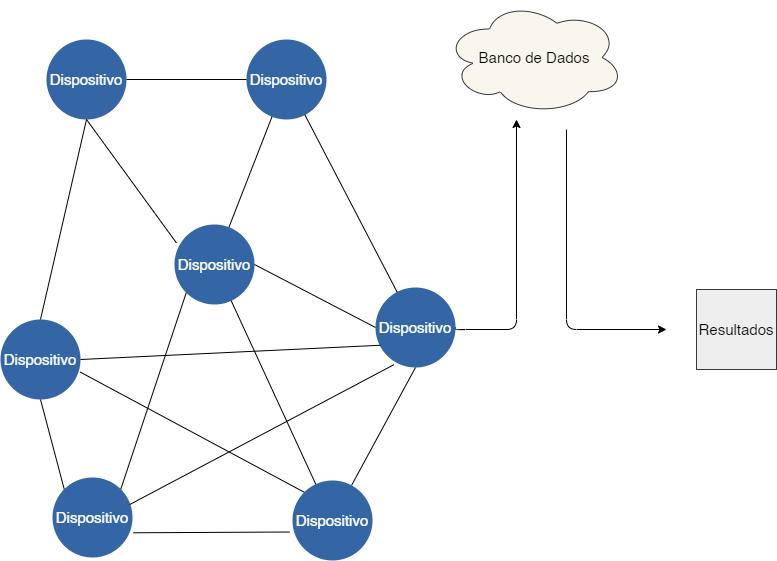
\includegraphics[width=\textwidth]{arq_rede}
    \caption{Arquitetura da rede de dispositivos}
    \label{fig:Diagrama de Blocos}
\end{figure}

\subsection{Banco de Dados}
Outro requisito comumente encontrado em dispositivos IoT focados em monitoramento é a alta disponibilidade de dados para que esse monitoramento em questão seja realizado de forma eficiente. Isso faz com que soluções de armazenamento em nuvem sejam boas alternativas, já que os dados estariam armazenados em um servidor externo ao sistema, possibilitando o seu acesso remotamente. Grandes empresas de tecnologia oferecem plataformas de desenvolvimento com interfaces de programação de aplicações (API, do inglês \textit{application programming interface}) que facilitam o desenvolvimento de bancos de dados conectados.

Para esse projeto, usaremos a solução AWS da Amazon, especificamente o serviço \textbf{AWS IoT Core} \cite{aws-iot}, que é um serviço que permite conexão de dispositivos a aplicativos em nuvem. Ele será utilizado em conjunto com o banco de dados NoSQL DynamoDB da própria plataforma.

% ========== Referências ==========
% --- IEEE ---
%	http://www.ctan.org/tex-archive/macros/latex/contrib/IEEEtran
%\bibliographystyle{IEEEbib}

% --- ABNT (requer ABNTeX 2) ---
%	http://www.ctan.org/tex-archive/macros/latex/contrib/abntex2
\bibliographystyle{abntex2-num}
%\bibliographystyle{plain}

\bibliography{reference_p1}


\end{document}
